% !TEX root = CSL 2021.tex


In the preceding section we showed how to associate each simple type $A$ with a  partial metric $d_{A}$ over the closed terms of type $A$. We now illustrate through a few basic examples how this metric can be used to formalize reasoning about program differences in a compositional way.




\subparagraph*{Taylor approximation}

Suppose that for all $n$, we can define a term $\mathtt T^{n}: ((\mathsf{Real}\to \mathsf{Real})\times \mathsf{Real})\to \mathsf{Real}\to \mathsf{Real}$ such that $\mathtt T^{n}\langle f, r\rangle$ computes the $n$-th truncated Taylor expansion of $f$ at $r$. 
Then, given a term $t[x]: \mathsf{Real}\to \mathsf{Real}$, the distance 
$d_{\mathsf{Real}\to \mathsf{Real}}(\mathsf C[t],\mathsf C[ \mathtt T^{n}\langle t,\mathtt 0 \rangle])$
between $t$ and its Taylor expansion within a context  $\mathsf C[\ ]= [\ ] r$ which applies them to some value $r$, can be computed as a function of the interval $[0,r]$.   
For instance, if $t[x]$ is some basic function, say $t[x]=\sin(x)$, using standard analytic reasoning we can compute a bound
$d_{\mathsf{Real}\to \mathsf{Real}}(\mathsf C[t],\mathsf C[ \mathtt T^{n}\langle t,\mathtt 0 \rangle])([0,r]  )\leq \frac{(d_{\mathsf{Real}}(0,r))^{n+1}}{(n+1)!} $.

\begin{remark}
If, instead, we had considered the $\sup$-distance for $\mathsf{Real}\to \mathsf{Real}$, \emph{i.e.} the distance $d_{\sup}(t[x],u[x])= \sup\{d_{\mathsf{Real}}(t[r], u[r])\mid r\in \mathsf{Real}\}$, then the reasoning above would be trivialised since we would have that 
$d_{\sup}(\sin(x), \mathsf T^{n} \langle \sin(x),0\rangle)=\infty$ (as illustrated in Fig. \ref{fig:sintaylor}).  
\end{remark}

\begin{figure}
\begin{subfigure}{0.5\textwidth}
\parbox[h][3.5cm][c]{\textwidth}{
\adjustbox{center}{$
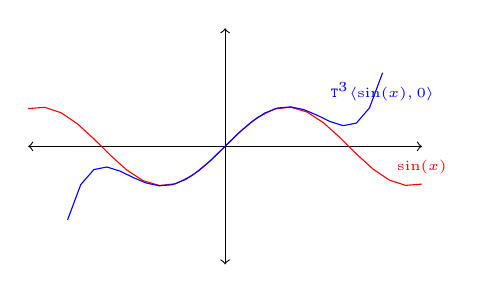
\begin{tikzpicture}[domain=-5:5, scale=0.5]
%\draw[very thin,color=gray] (-0.1,-1.1) grid (3.9,3.9);
\draw[<->]   (-5,0) -- (5,0);
\draw[<->] (0,-3) -- (0,3); % node[above] {$f(x)$};

   % \node at (0,0)[circle,fill,inner sep=1pt]{};
%
\draw[color=red, domain=-5:5] plot (\x, {sin(\x r) } ) node[above] {\tiny$\sin(x)$};

\draw[color=blue, domain=-4:4] plot (\x,{\x -((\x)^3)/6 + ((\x)^5/120  } ) node[below] {\tiny$\mathtt T^{3}\langle\sin(x),0\rangle$};


\end{tikzpicture}$}
}
\caption{\small The $\sup$-distance between $\sin(x)$ and its Taylor expansion $\mathtt T^{3}\langle\sin(x),0\rangle$ diverges.}
\label{fig:sintaylor}
\end{subfigure} \ \ \ 
\begin{subfigure}{0.45\textwidth}
\parbox[h][3.5cm][c]{\textwidth}{
\adjustbox{scale=0.55}{$
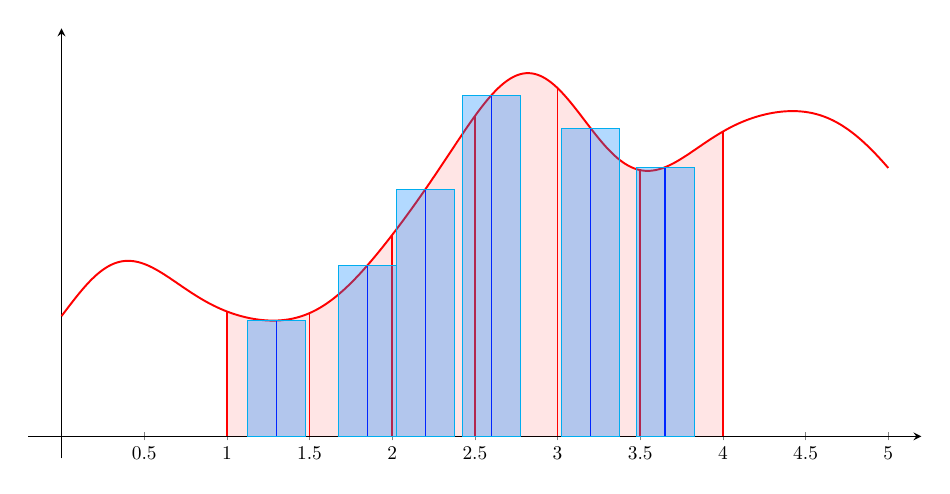
\begin{tikzpicture}[scale=0.7,
    declare function={
        f(\x)=2+sin(deg(\x-2))+sin(deg(3*\x))/2+sin(deg(5*\x))/8 + sin(deg(7*\x))/28;
    }
]
\begin{axis}[
    axis lines = middle,
    %xtick ={1,1.5,2,2.5,3,3.5,4},
    ytick ={0},
    %xticklabels = {$a=x_0$,$x_1$,$x_2$,$x_3$, $\ldots$, $x_{n-1}$,$x_n=b$},
    ymin = -0.2,
    ymax = 3.7,
    xmin = -0.2,
    xmax = 5.2,
    x=3cm,y=2cm,
    axis line style = thick,
    %xlabel={$x$},
    %ylabel={$y$},
    %extra x ticks={1.3,1.85,2.2,2.7,3.2,3.75},
%extra x tick labels={$\xi_1$, $\xi_2$, $\xi_3$, $\xi_4$, $\xi_{n-1}$, $\xi_n$},
]

\addplot [
    domain=1:4,
    samples=300,
    line width=1pt,
    fill=red, draw=none,
    fill opacity=0.1
] {f(x)} \closedcycle;

\addplot [
    domain=0:5,
    samples=300,
    line width = 1pt, red] {f(x)};

\addplot [
    ycomb, thick, red,
    no markers,
    samples at={1,1.5,...,4}
] {f(x)};

\addplot [
    ycomb, thick, blue,
    no markers,
    samples at={1.3,1.85,2.2,2.6,3.2,3.65}
] {f(x)};

\addplot[ybar, bar width=30pt, domain=1:4,
samples at={1.3,1.85,2.2,2.6,3.2,3.65}, fill=blue!50!cyan,fill opacity=0.3, draw=cyan]
  {f(x)};


\end{axis}
\end{tikzpicture}$}
}
\caption{\small Real integral $vs$ Riemann sum. \\ TO BE FIXED }
\label{fig:sintaylor}
\end{subfigure}
\end{figure}


\subparagraph*{Integral approximation}
A second natural example is numerical integration. Suppose that all functions in $\mathcal F_{n}$ are integrable and suppose we have at our disposal a term $\mathtt I_{r,s}: (\mathsf{Real}\to \mathsf{Real})\to \mathsf{Real}$ such that $\mathtt I_{r,s}f$ is (a precise enough approximation of) the definite integral $\int_{s}^{r}f(x)dx$.
In many contexts we might prefer to replace the expensive computation of $\mathsf I_{r,s}f$ by the (more economical but less precise) computation of a finite Riemann sum $\mathsf R^{n}_{r,s}f=  \sum_{i=1}^{n}(f x_{i})\cdot \Delta x$, where $\Delta x= |r-s|/n$ and $x_{i}= r+ i\cdot \Delta x$. 
It is well-known that the distance between the exact integral (that we suppose $\mathtt I_{r,s}$ is close enough to) and its approximation through a finite Riemann sum can be computed as a value $H(f'', n)$ depending on the second derivative of $f$ and $n$, that is
$d_{\mathsf{Real}}(\mathsf I_{r,s}f, \mathsf R^{n}_{r,s}f)\leq H(f'',n)$.

A bit more generally, we can consider the problem of bounding, given \emph{different} terms $f,g:\mathsf{Real}\to \mathsf{Real}$, the distance between the real integral of $\mathtt I_{r,s}f$ of $f$ and the approximate integral $\mathtt R^{n}_{r,s}g$ of $g$, supposing $f$ and $g$ are close each other on the interval $[r,s]$. 
 In fact, by standard calculation we can compute the bound
$d_{\mathsf{Real}} ( \mathsf{R}^{n}_{r,s}f, \mathsf R^{n}_{r,s}g)\leq 
d_{\mathsf{Real}\to\mathsf{Real}}(f, g)([r,s]) \cdot n (\Delta x)^{n}
$, which is small for small values of $|r-s|$. Then,
 using the triangular inequality we obtain an explicit bound
$d_{\mathsf{Real}} ( \mathsf{I}_{r,s}f, \mathsf R^{n}_{r,s}g)\leq
 d_{\mathsf{Real}} ( \mathsf{I}_{r,s}f, \mathsf R^{n}_{r,s}f)+
  d_{\mathsf{Real}} ( \mathsf{R}^{n}_{r,s}f, \mathsf R^{n}_{r,s}f)\leq 
 H(f'',n)+
d_{\mathsf{Real}\to\mathsf{Real}}(f, g)([r,s]) \cdot n (\Delta x)^{n}
$.

As in the previous example, we could not use the distance between $f$ and $g$ in a relevant way if this were the $\sup$-distance, since, although close on $[r,s]$, $f$ and $g$ might get arbitrarily far from each other over all reals. 



\subparagraph*{Loop perforation}
By adapting an example from \cite{chaudhuri}, we discuss a simplified example of the transformation which replaces $n$-iterations by $\lceil n/k \rceil$ iterations, in which only the iterations of $k\cdot i$ are performed and repeated $k$ times. 


Let $\mathsf{Nat}_{A}$ be a suitable type representing natural numbers in $\STLC$ and suppose  $t: (A\times A\to A) \to \mathsf{Nat}\to (A\to A)\to A$, for $n\geq 1$, is a term such that $th\mathtt n f$ 
computes the $n$-times iteration of $h$ as follows: $th \mathtt 0f= h\langle f\mathtt 0, f\mathtt 0\rangle$ and $th(\mathtt{n+1})f=h(th\mathtt n f, f\mathtt{n+1})$. 
Let $\mathsf{Perf}^{k}(t)$, the $k$-th perforation of $t$, be the function 
$\mathsf{Perf}^{k}(t)h\mathtt nf= t(\lambda x. (h^{(k)}x)) \mathtt{\lfloor n\rfloor_{k}} (\lambda x. f(x\cdot k)$, where $\lfloor n\rfloor_{k}$ indicates the least $m\leq n$ such that $m$ is divisible by $k$. 
It can then be checked that the distance 
$d_{A}(th\mathtt n f,  \mathsf{Perf}^{k}(t)h\mathtt nf  )$ between $t$ and its perforation can be bounded by 
computing the diameter of $\partial(t)   \partial(h) \tointerval{\mathtt n} (\lambda x.\partial (f)([\lfloor x/k\rfloor, x]))$.

%{
%
%given by $\mathsf{Perf}^{k}(t^{0})f= t^{0}f$ and $\mathsf{Perf}^{k}(t^{n+1})f=
%h( \mathsf{Perf}^{k}(t^{n})f, f \mathtt{\lfloor n+1/k\rfloor})$ if ${\lfloor n+1/k\rfloor}> {\lfloor n/k\rfloor}$, and $\mathsf{Perf}^{k}(t^{n+1})f=\mathsf{Perf}^{k}(t^{n})f$ otherwise.
%
%
%While $d_{A}(t^{1}f, \mathsf{Perf}^{k}(t^{1}f))$ is the self-distance of $t^{1}f\oeq_{\mathsf{A}}f\mathtt 0$ (which is equal to $0$ if, say, $A=\mathsf{Real}$), f

%
%
%As soon as we have a bound  $\rho: a,\mathtt n \mapsto \partial(h)(a,\tointerval{\mathtt n}) \vee a$
% for the smallest interval containing a value $t:A$ and its image $h(t,\mathtt n)$, we  can  compute explicit bounds for  the distance $d_{A}(t^{n}f,\mathsf{Perf}^{k}(t^{n})f)$. In fact, by letting $D_{A}(u,v): a\mapsto \tointerval u\vee \tointerval v$ and recalling that $d_{A}(u,v)=\diam_{A}(D_{A}(u,v))$, we can use the following lemma. 
%\begin{lemma}
%$D_{A}(t^{n+1}f, \mathsf{Perf}^{k}(t^{n+1})f)\leq H(n, \rho, \partial(h), \partial(f), D_{A}(t^{n}f,  \mathsf{Perf}^{k}(t^{n})f))$, where 
%%$\phi=d_{\mathsf{Real}\to \mathsf{Real}}(h,h)$, $\psi= d_{\mathsf{Real}\to \mathsf{Real}}(f,f) $ and , where $H(\phi,\psi,\Phi) $ is
%$H(n,\rho,\phi,\psi, \chi)=
%  \rho^{n}(\tointerval{f\mathtt 0})
%  +
%  \chi
%  +
% \psi( \chi, \psi (\mathtt{n+1},\mathtt{ \lfloor n+1/k\rfloor} ))
%$ and $\rho^{n}(a)$ is defined by $\rho^{0}(a)=a$ and $\rho^{n+1}(a)=\rho(\rho^{n}(a),\mathtt n)$.  
%%
%%In fact, since $t^{n+1}f= h \langle t^{n}f,  f\mathsf{n+1}  \rangle$ and 
%%$\mathsf{Perf}^{k}(t^{n+1})f$ is either equal to $\mathsf{Perf}^{k}(t^{n})f$, if $\lfloor n+1/k\rfloor=\lfloor n/k\rfloor$, or 
%%to $ h\langle \mathsf{Perf}^{k}(t^{n}f),  f\mathsf{\lfloor n+1/k\rfloor}  \rangle$, we have
%%$d_{A}(t^{n+1}f, \mathsf{Perf}^{k}(t^{n+1}f)) \leq d_{A}(t^{n+1}f, \mathsf{Perf}^{k}(t^{n}f)) +
%%d_{A\times A\to A}(h,h)( D_{A}( t^{n}f, \mathsf{Perf}^{k}(t^{n}f)),\partial(f)( a_{n,k}) )
%%$
%%where $a_{n,k}$ is the interval
%%$\big [ \mathtt{n+1},  \mathtt{\lfloor n+1/k\rfloor}\big ]_{A}$. 
%
%
%
%\end{lemma}
%\begin{proof}
%Computations are done in the appendix [ADD THEM].
%\end{proof}
%}
%




